\documentclass[12pt]{article}
\usepackage{graphicx}
\usepackage{setspace}
\usepackage[margin=1in]{geometry}	% Page margins
\usepackage[]{natbib}
\doublespacing
\begin{document}

\author{Samuel Leeman-Munk}
\date{\today}
\title{A Prolog-based Natural Language Database \\ with Procedural Frontend}
\maketitle
\abstract{A Natural Language Queriable Database is a collection of knowledge that a user can gain knowledge from much like he or she might ask another human being. Although the ultimate vision of a Natural Language Database (NLD) is still in the realm of science fiction, Natural Language Databases of varying ability do exist today, and many other well-known software such as Google and Wolfram Alpha use Natural Language techniques in helping their users get what they want.

Prolog is a declarative logic programming language associated with both Natural Language Analysis and Artificial Intelligence, making it a prime candidate for both parsing natural language queries and finding answers to them. This paper discusses a theoretical NLD that uses two Prolog databases: one English language parsing database and one database of information. These databases are connected with an imperative front-end, in this paper Perl.}
\clearpage
\section*{Introduction}
Imagine 24-hour customer support with no hold time. Consider a doctor's office that can advise and assist at a professional medical level thousands of people at once. Think if instead of fumbling around on Google trying to get just the right search term, you just ask a question and have it instantaneously answered. Imagine a computer that is smart enough to tell you exactly what you want to know, rather than simply what you ask. These are the ultimate visions of the Natural Language Queriable Database. Unlike conventional databases that are accessed using algorithmic computer languages, a Natural Language Database (NLD) handles the translation from human language to computer language itself, allowing people with no technical skill to ask questions and get helpful answers.

Prolog, short for Programmation en Logique (programming in logic) was developed in the early 1970s as a processor for the French language, but has since become a language associated heavily with both natural language processing and artificial intelligence ~\citep{birthofprolog}. For this reason, Prolog seems a particularly elegant solution to an Natural Language Database, which uses both natural language processing and artificial intelligence in the process of understanding a question a user asks and finding the answer to that question. This paper explores the subjects of the Natural Language Database and Prolog in general, and specifically explores a Natural Language Database for English speakers that employs a procedural frontend connecting two Prolog programs -- one for natural language processing and one for intelligently finding answers to the disambiguated queries.

\section*{Algorithmic Language Parsing}
Unfortunately, translating even the simplest human question into something a computer can understand is non-trivial at best. Human languages are notorious for exceptions and inconsistencies that do not fall easily into algorithmic parsing. Linguistic anomalies, ambiguous questions, improperly formed questions with misspellings and grammatical errors, poorly worded questions, statements that imply questions, and questions that may in fact want something different from what they literally ask plague attempts at computationally understanding what a human asking a question really wants to know ~\citep{Jurafsky}.

For the above reasons, it seems to the casual observer that language recognition cannot be subjected to a deterministic process ~\citep{Marcus}. Indeed it's reasonable to believe that no algorithm of any complexity could have a 100 percent success rate communicating with humans - even humans fail to understand human speech now and then. An algorithm must make educated guesses as to the meaning of a human request, the accuracy of the guess increasing with the sophistication of the algorithm. Fortunately, despite their algorithmic shortcomings, natural human languages do have forms and structures that to a limited extent can be parsed into logical meaning. For a parser to understand the meaning of a human question as completely as possible, this is where to start.

The first logical step in making a language parsing algorithm is to separate the words into logical groups. Of course, the first and most appropriate grouping for natural language is parts of speech. Far more than merely the grade-school noun, verb, adjective, article, interjection and a few more, scholarly part-of-speech lexicons segregate words into many fields. From Penn Treebank's 45 to a staggering 146 in the C7 tagset, there's some disagreement as to exactly where one type of word ends and another begins. ''Tagging'' words with their parts of speech is the first step for syntactic language recognition, as part of speech more than anything else allows for predicting how words will fit together in a sentence and provides tremendous help in disambiguating word meaning ~\citep{Jurafsky}.

There are two supercategories of parts-of-speech: closed class and open class types. A closed class is one that is comparatively less likely to accept new members.  New prepositions, for example, are exceptionally rare in comparison to an open class part of speech such as nouns and verbs, which constantly accept new members, often borrowed from other languages (restaurant from French) or brought from other parts of speech ('to google'). Between spoken dialects and bodies of text, the set of open class words can vary dramatically, but large enough samples tend to share closed class words ~\citep{Jurafsky}. 

Open class types tend to hold the bulk of a sentence's meaning while closed class types tend to be "function words" that serve as abstract qualifiers and grammatical glue that holds the other words together. As an example of subdivisions in part of speech, Daniel Jurafsky and James H. Martin's \underline{Speech and Language Processing} divides the function words into prepositions(under, beside), articles(a, an, the), pronouns(she, his, what), conjunctions(and, but) auxiliary verbs(can, should, will), particles(down, off), and numerals(one, fifteen). Open class words tend to be nouns, verbs, adjectives and adverbs, each of which is further subdivided to varying extent depending on the opinions of the divider ~\citep{Jurafsky}.

Unfortunately, one word can exist in multiple parts of speech, and even with a completely divided and subdivided dictionary, it's generally not trivial to tag any given sentence. "Watch," for instance, can refer to a handheld timetelling device or someone's turn to stand guard, or it can refer to observing something over a period of time. "Watch my watch," could be noun-pronoun-noun, noun-pronoun-verb, verb-pronoun-noun or verb-pronoun-verb. Here an algorithmic parser can use a predefined set of rules to pick the most likely part of speech. For instance, watch can be either a main verb or a count noun, a non-proper noun that refers to a distinct object rather than a mass, such as water. Singular count nouns don't tend to begin sentences as they tend to follow an article so the watch at the beginning of the sentence is more likely a verb. This reduces the possibilities to verb-pronoun-verb or verb-pronoun-noun. "My" is a possessive pronoun, which tends to precede a noun (that which is possessed), so verb-pronoun-noun is the most reasonable interpretation.  Working with text by way of picking words and phrases based on the one preceding them is known as a Markov chain algorithm ~\citep{Markov}.

Tagging requires a ruleset, and different styles of tagging are separated by how the rules are decided. A Rule-based tagger gets its rules from a vast manually assembled database, while a stochastic tagger makes a table of rules from analyzing an already-tagged corpus of text ~\citep{Jurafsky}. While the former tends to be more reliable, it does not scale well. Manually encoding every grammatic possibility of the English language can become costly and time consuming. The latter can analyze a large corpus of text, but the corpus must already be tagged, which, except in the unlikely situation that another high-quality tagger is available, must also be done manually. In a Natural Language Database environment, a manually encoded ruleset that covers the most commonly used structures is sufficient. A full-featured NLD has other failsafes that can account for unrecognized grammars. 

Sometimes after the Markov Chain tagging process a word still has multiple possibilities. In this case, the word can have more than one tag ~\citep{Tomita}. This is clearly not preferable, and cannot be disambiguated without moving to a higher level of understanding. This new level of understanding will also help get meaning from complex sentences. A sentence like ''I really think that Tyler should start on that big project soon,'' contains structures poorly represented by just a list of parts of speech. We can move closer to solving the problem of ambiguity of individual words while also gaining an entirely new level of meaning by identifying entire phrases that behave as a particular word type in a group ~\citep{Jurafsky}. For instance, the above sentence nagging Tyler could be described in terms of the parts of speech of each of its lowest components, or at a higher level, it could be marked "noun phrase(I) verb phrase(really think) conjunction(that) noun phrase(Tyler) verb phrase(should start on that big project soon)." In fact, it could be marked any number of ways. The last big chunk could be split into smaller verb and noun phrases, the first parts could be put together, ''I'' could be separated as one noun phrase while the rest of the sentence gets lumped together into a verb phrase, or the whole sentence could just be marked ''sentence.'' The mathematical system for modeling phrase structures in this way is called ''Context-Free Grammar'' or more intuitively ''Phrase-structure Grammar'' ~\citep{Peters}. The specific rules for grammatical phrases differ depending on what list of part-of-speech tags is being used, but every proper system ends at the same result.

Naturally, just marking a sentence ''Sentence'' isn't particularly helpful. Separating it entirely into its lowest parts is moreso, but only marginally.  One option is to try and find a middle ground with the most meaningful possible structure, but what might be a better option would be to store all the levels, say, in a tree (\ref{fig:Phrase-Tree}). This system provides a more sophisticated level of understanding of sentence structure, and provides better information to help a parser derive useful meaning. For instance, three levels up from the bottom of the tree we can see the sentence as a noun phrase followed by a verb phrase, a form generally taken by declarative sentences. Similarly, ''Watch my watch'' maps out to be just one big verb phrase, suggesting an imperative statement, which a natural language database can then parse to find out if it can do what the user has told it to do~\citep{Jurafsky}. 

\begin{figure}[p]
	\centering
		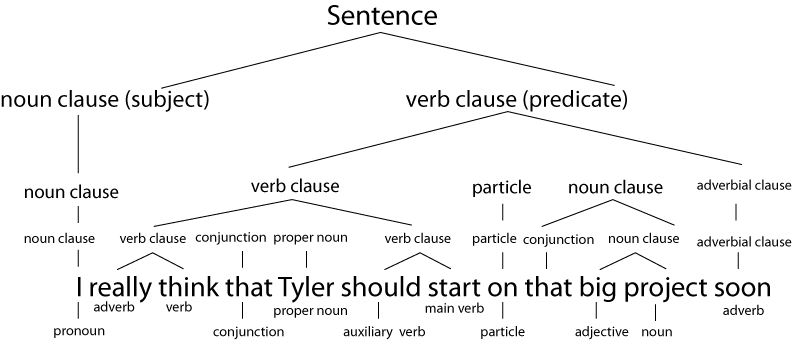
\includegraphics[width=13cm]{Phrase-Tree}
		\caption{One example of a parse tree}
	\label{fig:Phrase-Tree}
\end{figure}

It's a little more complicated to find a parse tree in a sentence than it is just to go through and tag word-by-word. The process can be thought of as a search algorithm that searches through the set of all possible trees to find the one that fits the sentence. We start knowing that the leaves at the bottom of the tree must be all of the words of the sentence in order, and that top of the tree must be a sentence, which breaks down in a certain fashion defined by the grammar of the language ~\citep{Jurafsky}.

There are two basic algorithms behind the parsing of sentences into parse trees. The first starts from the root node, the sentence, and works down, expanding through each possible expansion of a sentence, then recursively expanding each of the resulting partial trees through all their possibilities, until reaching the part-of-speech categories at the end. Then the resulting part-of-speech category sets are checked, and any that don't match the sentence are thrown out. The remaining trees (ideally tree) are the sentence's parse trees. Understandably, this is called the top-down algorithm. The second algorithm, the bottom-up algorithm, starts from the words and their tags themselves, and follow the rules backwards. Trees that make it to sentence are kept as parse trees and the rest are tossed. In both cases, ambiguous sentences that return multiple parse trees can be disambiguated by linguistic heuristics or selected later by whether the artificial intelligence section of the database thinks they make sense. ~\citep{Tomita}

The top-down tree and the bottom-up tree each have their strengths and weaknesses. A strictly bottom-up algorithm can take the input and build partial trees that cannot even fit with their immediate neighbors, let alone the sentence at the top, while a strictly top-down algorithm generates all the trees that can possibly be made by the grammar before even looking at the input. Neither of these approaches takes complete advantage of both the grammars and input words ~\citep{Jurafsky}.

Most modern parsers use a combination of the top-down and bottom-up approaches. For example, by looking at the left corner, or the leftmost leaf of the tree, i.e. the first word of the sentence, we can cancel certain sentence types from the start, dramatically reducing the number of trees a top-down parser will need to search through. ''I really think that Tyler should start on that big project soon,'' starts with ''I,'' a pronoun, which can only be the start of a noun phrase, meaning the sentence cannot take the Verb phrase form of imperative, nor can it start with an auxiliary verb (can,should) to form a yes-or-no question, so those and other similarly ill-fitting trees can be cut out before expanding, reducing the workload by more than two thirds ~\citep{Jurafsky}.

The simple CFG-based grammar as we have described it does not cover grammatical agreement. A grammatical detail as minor as the difference between ''he eats'' and ''he eat'' would at a glance not seem to bear particularly heavily on language comprehension and understanding, but Manny Rayner et al. conducted a study in 2000 suggesting just the opposite. Rayner found that CFG-based English language recognition in two separate systems had a significantly lower rate of semantic error when taking into account grammatical agreement ~\citep{Rayner}.

A CFG-based grammar can be designed to cover grammatical agreement, but it would require making a new phrase for each combination set of agreements. A simple verb clause would need to be expanded into a singular past verb clause, a singular present verb clause, a singular infinitive verb clause, a plural past verb clause and so on, and that's not even taking mood into account. For this reason, we can use a more compact formalism based on the CFG, a Definite Clause Grammar (DCG) works very much like a CFG except that a clause can have multiple variables in addition to its identifier. A verb clause, then, has values denoting its mood, tense, and number, that affects the valid moods, tenses, and numbers of its sub-clauses. DCGs also introduce context-dependency and allow for even better translation into meaning. DCGs have been used to make many language parsing algorithms for both natural languages and programming languages ~\citep{DCGNLA}.

\section*{Prolog as a Natural Language Parser}

Prolog's relationship with DCGs is hardly a new one. In fact, it's difficult to mention one without the other coming up, especially in the context of natural language analysis. Prolog handles DCGs natively, and can parse them on its own.

\singlespacing
\bibliography{capstone}{}
\bibliographystyle{plainnat}
\end{document}